\section{538 --- Convert BST to Greater Tree}
Given a Binary Search Tree (BST), convert it to a Greater Tree such that every key of the original BST is changed to the original key plus sum of all keys greater than the original key in BST.

\paragraph{Example:}

\begin{flushleft}
\textbf{Input}: The root of a Binary Search Tree like this:

\begin{figure}[H]
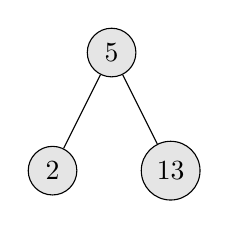
\begin{tikzpicture}
[every node/.style={draw, circle, fill=gray!20!, minimum size=5mm}]

\node{5}
child {node{2}}
child {node{13}};

\end{tikzpicture}
\end{figure}


\textbf{Output}: The root of a Greater Tree like this:

\begin{figure}[H]
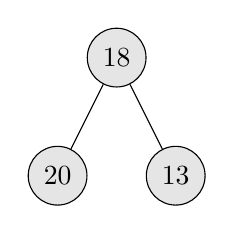
\begin{tikzpicture}
[every node/.style={draw, circle, fill=gray!20!, minimum size=5mm}]

\node{18}
child {node{20}}
child {node{13}};

\end{tikzpicture}
\end{figure}

\end{flushleft}
